\noindent
Graph processing is a critical component in a broad range of applications ranging from social network analysis, medical diagnostics, and drug interaction studies.  
Given the vast size of these graphs with billions of edges and vertices, graph algorithms stress memory and scaling capabilities of computing systems. 
In this proposal we treat graph algorithms as linear algebraic problem formulations, where graphs are represented as adjacency matrices.  
The evolving duality between graph algorithms and their equivalent matrix operations forms a solid basis for 
designing computing systems %that can efficiently manipulate matrix operations.  
for efficient graph processing~\cite{graph:primitives}.
For example, there are well known linear algebraic problem formulations for graph algorithms such as breadth first search, strongly connected components, shortest path, stress centrality, betweenness centrality, sub-graph detection and so on.  
These algorithms demand a diverse range of matrix operations, including matrix multiplication, Kronecker product,  matrix decomposition, inner and outer products, matrix inversion, matrix transpose and Eigen value computation.  
Supporting such a broad range of operations on extremely large matrices is the first challenge that will be tackled in this proposal. 


%An equally daunting challenge is the representation of large graphs as adjacency matrices in memory.
Given the diversity of application domains where graph analytics may be used, the structure of graphs may also be varied. 
To improve storage and bandwidth efficiency, sparse graphs may be stored in  a (double) compressed sparse row (CSR) or column (CSC) format. 
%But sparse graph representations also worsen irregular access patterns to memory.
%M - I revise this because reading non-zero elements is sequential memory accesses. However, the last part of sparse matrix operations (merging processes) are very irregular. 
%But sparse graph operations involve a large number of irregular memory accesses.
But sparse matrix operations involve a large number of irregular memory accesses.
Some graphs may exhibit power law distributions where only a few vertices contribute to most edges in the graph. 
Such disparity leads to significant load imbalances in computations.  
Efficiently handling both sparse and dense matrices with varying degrees of connectivity is the second challenge tackled in this proposal. 

 
Finally, scaling the execution of linear algebraic manipulations, through parallelization, while mitigating Amdahl's bottleneck is another challenge that this proposal tackles. 
Parallel execution of matrix operations can be mapped to various distributed computing paradigms, such as Spark~\cite{zaharia2010spark, MapReduce}, Pregel~\cite{pregel, Giraph} and Parallel-R~\cite{kabacoff2015r}. 
For instance, many PGAS (partitioned global address space) approaches distribute the equal number of vertices across nodes (equal number of rows from the adjacency matrix). 
However, when vertex degrees exhibit power law distribution, it is extremely difficult to balance the load across computational nodes. 
Launching a new iteration of the computation requires the previous iteration to complete, thereby forcing a barrier synchronization across various threads. 
In the presence of load imbalances such synchronizations curtail scaling. 


These observations lead to the main research thrusts of this proposal, as described below. 
To guide the discussion of the proposed research, we first present an overview of the system architecture that we will design and build. 
The system will rely on processing-in-memory architecture, but appropriately adapted for sparse matrix operations for graph processing. 
Fig.~\ref{fig:arch}(a) presents the overview of the GAMA (Graph Acceleration through Matrix Abstraction) system consisting of 16 GAMA tiles and host systems connected by power-efficient inter-chip OpenCAPI links.
A GAMA tile consists of a many-core GAMA accelerator, four 8GB high-bandwidth memory dies (DiRAM4) with 64$\times$32-bit memory channels, 
and four OpenCAPI links with aggregate memory bandwidth of 1TBps to four other GAMA tiles or a host system.
Subsequently, we will describe the detail of the accelerator (cf. Sec.~\ref{sec:processing}),  memory sub-system (cf. Sec.~\ref{sec:memory}), and circuit support for efficient inter-chip communication and strong scaling over 16 GAMA tiles (cf. Sec.~\ref{sec:scale}).


\begin{figure}
\center
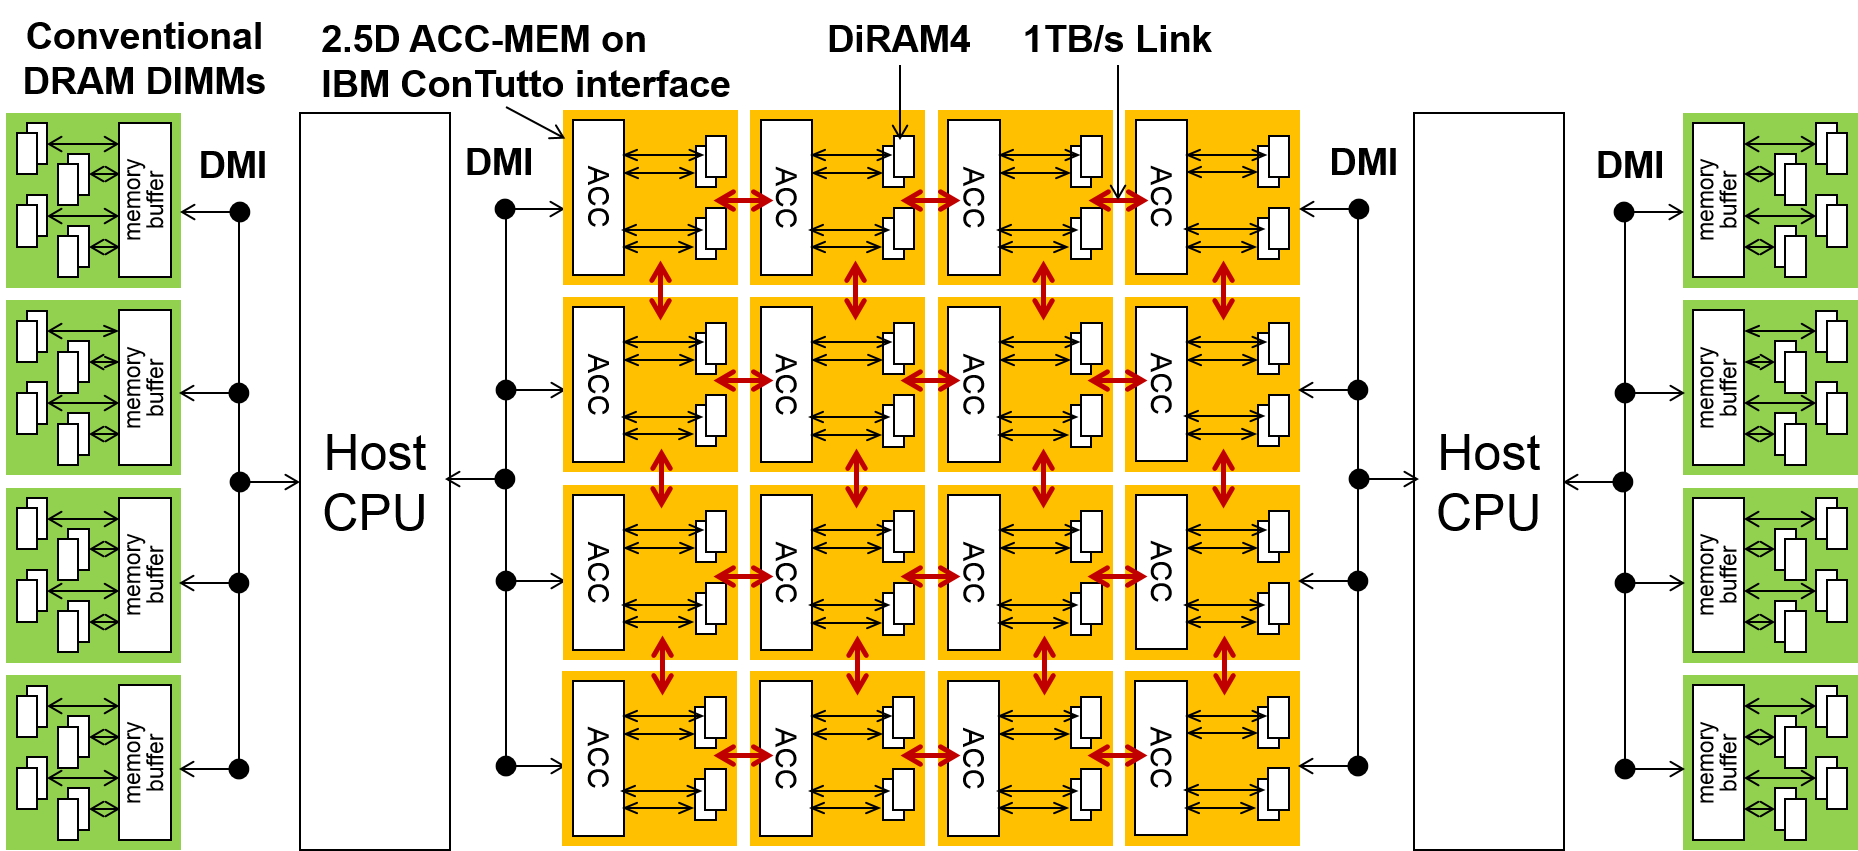
\includegraphics[width=1.0\linewidth]{fig/arch.png}
\caption{GAMA (a) system architecture, (b) accelerator architecture (the left-top cluster), (c) core microarchitecture with a 8-lane sparse matrix acceleration engine.}
\label{fig:arch}
\end{figure}


